\documentclass[a4paper,11pt,twoside]{article}
%\documentclass[a4paper,11pt,twoside,se]{article}

\usepackage{UmUStudentReport}
\usepackage{verbatim}   % Multi-line comments using \begin{comment}
\usepackage{courier}    % Nicer fonts are used. (not necessary)
\usepackage{pslatex}    % Also nicer fonts. (not necessary)
\usepackage[pdftex]{graphicx}   % allows including pdf figures
\usepackage{listings}
\usepackage{pgf-umlcd}
\usepackage{blindtext}
\usepackage{enumitem}
%\usepackage{lmodern}   % Optional fonts. (not necessary)
%\usepackage{tabularx}
%\usepackage{microtype} % Provides some typographic improvements over default settings
%\usepackage{placeins}  % For aligning images with \FloatBarrier
%\usepackage{booktabs}  % For nice-looking tables
%\usepackage{titlesec}  % More granular control of sections.

% DOCUMENT INFO
% =============
\department{Department of Computing Science}
\coursename{Parallel Programming 7.5 p}
\coursecode{5DV152}
\title{Exercises, Chapter/Topic 5}
\author{Lorenz Gerber ({\tt{dv15lgr@cs.umu.se}} {\tt{lozger03@student.umu.se}})}
\date{2017-02-03}
%\revisiondate{2016-01-18}
\instructor{Lars Karlsson / Mikael Ränner}


% DOCUMENT SETTINGS
% =================
\bibliographystyle{plain}
%\bibliographystyle{ieee}
\pagestyle{fancy}
\raggedbottom
\setcounter{secnumdepth}{2}
\setcounter{tocdepth}{2}
%\graphicspath{{images/}}   %Path for images

\usepackage{float}
\floatstyle{ruled}
\newfloat{listing}{thp}{lop}
\floatname{listing}{Listing}



% DEFINES
% =======
%\newcommand{\mycommand}{<latex code>}

% DOCUMENT
% ========
\begin{document}
\lstset{language=C}
\maketitle
\thispagestyle{empty}
\newpage
\tableofcontents
\thispagestyle{empty}
\newpage

\clearpage
\pagenumbering{arabic}

\section{Introduction}
This report is part of the mandatory coursework. It describes the solutions for several chosen exercises from the course book \cite{pacheco2011}.

\section{Identities for various reduction operators - 5.4}

The identity values for various operators are shown in table \ref{tab:identity}.

\begin{table}[]
  \centering
  \caption{This table shows the identity values for various operators in C}
  \label{tab:identity}
  \begin{tabular}{cc}
    \multicolumn{1}{l}{operator} & \multicolumn{1}{l}{identity value} \\ \hline
    \&\&                         & 1                                  \\
    ||                           & 0                                  \\
    \&                           & $\sim$0                            \\
    |                            & 0                                  \\
    \textasciicircum             & 0
  \end{tabular}
\end{table}

\section{Rounding errors - 5.5}
It was assumed that in this exercise, one does not have to worry about how floats actually are represented in computers with sign, exponent and signigicant field.
The interpretation is just based on how many digits are used to represent the given numbers. Hence in a), the sequence of values in the variable sum is ${0.0, 2.0, 4.0, 8.0, 1010.0}$. The last value is based on the fact that 1008.0 will be rounded from four digits in the register to 1010 with 3 digits in the variable.
For b), sum of thread 0 is ${0.0, 2.0, 4.0}$, and sum for thread 1 is ${0.0, 4.0, 1000.0}$. After the reduce of sum from both threads, sum will be $1000$.

It can be seen that the results from serial and parallel computation differ. This is because for floats, the sequence of addition matters when values are rounded due to too high precision. 

\section{Default scheduling - 5.6}
A program was written to obtain the default scheduling of MP in for loops. Instead of indicating a range, indivdual indices for each thread are given. This is more flexible for various thread/iteration combinations when one thread can process two sequences of indices that don't follow each other. The source code can be found in appendix \ref{app:default}.  

\section{Loop-carried dependence - 5.8}
Here the problem of loop-carried dependence can be solved by looking at the actual function or values that result. Instead of using `back' indices, a more explicit form can be written:
\begin{equation}
(\frac{i}{2} + 0.5)\times i  
\end{equation}

\section{Thread-safe string tokenizer - 5.16}
Here it was asked to provide a string tokenizer that is thread save and does not modify the input string.
A wrapper function was written around the thread-save string.h library function strtok\_t to provide a version that does not modify the input string. Find below the source code:
\begin{verbatim}
char *tokenizer(char *str, const char *delim, char **saveptr){
  char *token;

  if(str != NULL){
    char *copied_str = malloc(strlen(str + 1));
    strcpy(copied_str, str);
    token = strtok_r(copied_str,delim, saveptr);
  } else {
    token = strtok_r(NULL, delim, saveptr); 
  }

  return token; 
}
\end{verbatim}

\section{Histogram A5.1}
Here, it was asked to use OpenMP to make a parallel version of the histogram program in chapter 2. The given serial code from chapter 2 was modified by including \verb+#pragma omp parallel for+ above the main 'work' for loop. The source code of the modified \verb+main+ function can be found in appendix \ref{app:histo}. This exercise seems to serve as a good example of how quick and easy some serial programs can be made parallel by using OpenMP.


\section{Count sort A5.3}
\begin{enumerate}[label={\alph*)}]
\item the variables \verb+i+ and \verb+count+ should be made private.
\item No, there are only data dependences left, but by setting private the above mentioned variables, there are no loop-carried dependences left. 
\item It would be possible to make memcpy parallel by parametrizing the arguments:
\begin{verbatim}
for (i = 0; i < n; i++) {
    memcpy((a+i), (temp+i), sizeof(int));
}
\end{verbatim}
  
\item A parallel version of the `Count\_sort' sort algorithm was implemented using OpenMP. The source code can be found in Appendix \ref{app:countsort}.
  
\item For a quick comparison of the performance, a serial implementation with countsort and one with the quicksort library function were compared on a random array with 1000 entries and boxplotted in figure \ref{fig:countsort}. It is obvious that under the tested parameters, `quicksort' outperforms also the parallel OpenMP implementation. The OpenMP implementation shows compared to the serial algorithm a reasonable speed-up for 2 and 4 threads. Then the curve flattens out. Benchmarking was run on a 4 core Probably, benchmarking also for larger arrays would establish again better speed-ups. Without having tested for it, I would expect this implementation to be weakly scalable in a reasonable range.  
\end{enumerate}

\begin{figure}

  \centering
  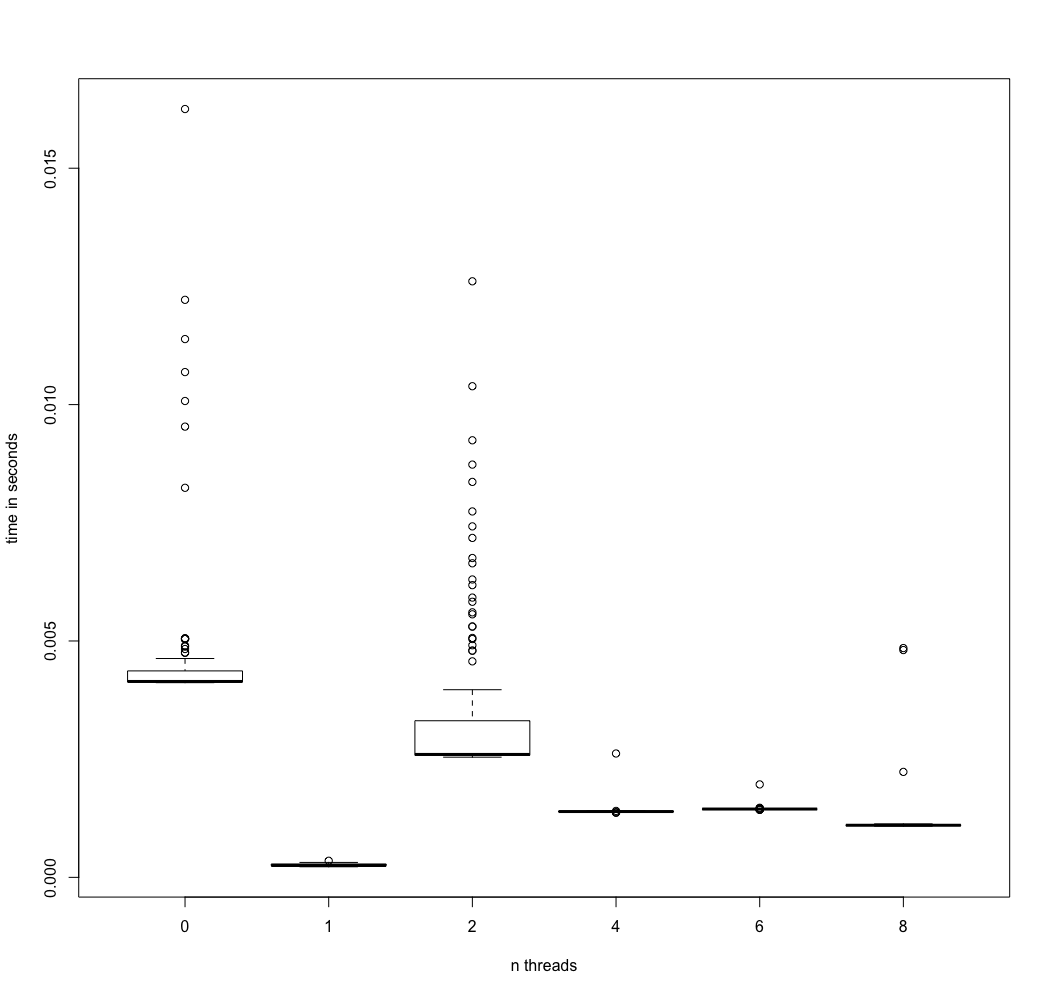
\includegraphics[width=1\textwidth]{countsort.png}
  \caption{\textit{This boxplot shows the comparison of the parallel OpenMP count sort implementation (n = \{2, 4, 6, 8\} with the serial countsort (n = 0) and with using the serial quicksort library function (n = 1). It is quite obious that quicksort outperforms also the parallel OpenMP implementation.}}
  \label{fig:countsort}
\end{figure}




\section{Backward substitution A5.4}
\begin{enumerate}[label={\alph*)}]
\item outer of row-oriented can not be parallelized
\item inner for loop of row-oriented backward substitution is basically a reduce operation onto an array. Hence it can be parallelized.
\item the second outer loop of the column-oriented can not be parallelized
\item the inner loop of the column-oriented can be parallelized
\item Program
\item Schedule
\end{enumerate}


\appendix

\section{C Source Code of Exercise 5.6}{\label{app:default}}
\begin{verbatim}
/**
 * omp_default.c
 * 
 * MP program to determine standard 
 * distribution of threads to for
 * loop indices.
 * @usage ./omp_default <threads> <iterations> 
 */
#include <stdio.h>
#include <stdlib.h>
#include <omp.h>

int main(int argc, char* argv[]){
  int thread_count, iterations, i, j;
  int *assignments;
  int my_rank;

  thread_count = strtol(argv[1], NULL, 10);
  iterations = strtol(argv[2], NULL, 10);

  assignments = (int*) malloc(iterations * sizeof(int));

  # pragma omp parallel for num_threads(thread_count)
  for(i = 0; i < iterations; i++){
    my_rank = omp_get_thread_num();
    assignments[i] = my_rank;
  }

  for(i = 0; i < thread_count; i++){
    printf("Thread %d: Iterations ", i);
    for(j = 0; j < iterations; j++){
      if(assignments[j] == i){
	printf("%d ", j);
      }
    }
    printf("\n");
  }

  return 0;
}

\end{verbatim}

\section{C Source Code of Exercise A5.1}{\label{app:histo}}

\begin{verbatim}
#include <stdio.h>
#include <stdlib.h>
#include <omp.h>

int main(int argc, char* argv[]) {
   int bin_count, i, bin;
   float min_meas, max_meas;
   float* bin_maxes;
   int* bin_counts;
   int data_count;
   float* data;
   int thread_count;

   /* Check and get command line args */
   if (argc != 6) Usage(argv[0]); 
   Get_args(argv, &bin_count, &min_meas, &max_meas, &data_count);
   thread_count = strtol(argv[5], NULL, 10);

   /* Allocate arrays needed */
   bin_maxes = malloc(bin_count*sizeof(float));
   bin_counts = malloc(bin_count*sizeof(int));
   data = malloc(data_count*sizeof(float));

   /* Generate the data */
   Gen_data(min_meas, max_meas, data, data_count);

   /* Create bins for storing counts */
   Gen_bins(min_meas, max_meas, bin_maxes, bin_counts, bin_count);

   /* Count number of values in each bin */
#  pragma omp parallel for num_threads(thread_count)
   for (i = 0; i < data_count; i++) {
      bin = Which_bin(data[i], bin_maxes, bin_count, min_meas);
      bin_counts[bin]++;
   }

#  ifdef DEBUG
   printf("bin_counts = ");
   for (i = 0; i < bin_count; i++)
      printf("%d ", bin_counts[i]);
   printf("\n");
#  endif

   /* Print the histogram */
   Print_histo(bin_maxes, bin_counts, bin_count, min_meas);

   free(data);
   free(bin_maxes);
   free(bin_counts);
   return 0;

}  /* main */
\end{verbatim}



\section{C Source Code of Exercise A5.3}{\label{app:countsort}}
\begin{verbatim}
/**
 * omp_countsort.c
 * 
 * OpenMP implementationof count sort algorithm
 * @usage ./omp_countsort <threads> <data_count>
 */
#include <stdio.h>
#include <stdlib.h>
#include "timer.h"
#include <omp.h>
#include <string.h>


void Count_sort (int a [], int n , int thread_count);

int main(int argc, char *argv[]){

  int thread_count, i;
  int *test;
  int data_count = strtol(argv[2], NULL, 10);
  double start, finish;

  test = (int*) malloc(data_count*sizeof(int));
    
  srand(0);
  for (i = 0; i < data_count; i++)
    test[i] = rand()%101;

  thread_count = strtol(argv[1], NULL, 10);

  for(int i = 0; i < data_count; i++){
    printf("%d ", test[i]);
  }
  printf("\n");

  GET_TIME(start);
  Count_sort(test, data_count, thread_count);
  GET_TIME(finish);

  for(int i = 0; i < data_count; i++){
    printf("%d ", test[i]);
  }

  printf("\n");

  printf("%e\n", (finish - start));

  return 0;
}


void Count_sort (int a [], int n , int thread_count) {
  int i, j , count;
  //int my_rank = omp_get_thread_num();
  
  int* temp = malloc ( n *sizeof(int));

# pragma omp parallel for num_threads(thread_count) \
  private(j, count)
  for ( i = 0; i < n ; i ++) {
    count = 0;
    for ( j = 0; j < n ; j ++)
      if ( a[j] < a[i])
	count ++;
      else if (a[j] == a[i] && j < i )
	count ++;
    temp[count] = a [i];
  }
  
# pragma omp parallel for num_threads(thread_count)
  for (i = 0; i < n; i++) {
    memcpy((a+i), (temp+i), sizeof(int));
  }


  free ( temp );
}


\end{verbatim}

\addcontentsline{toc}{section}{\refname}
\bibliography{references}

\end{document}
